\newpage
\subsection{Algorithms in Graph}


\begin{minipage}{.5\linewidth}
    \den{Cut}{
        A cut is a partition of the vertices of a graph into two disjoint subsets.
        Any cut determines a cut-set, the set of edges that have one endpoint in
        each subset of the partition. These edges are said to cross the cut. In a
        connected graph, each cut-set determines a unique cut, and in some cases
        cuts are identified with their cut-sets rather than with their vertex
        partitions.
    }\label{definition:cut_graph_theory}
\end{minipage}\hfill%
\begin{minipage}{.49\linewidth}
    \begin{figure}[H]
        \begin{center}
            \subfloat[Minimum Cut]{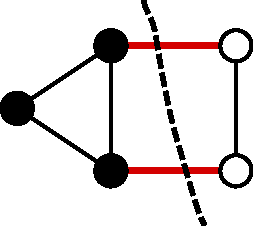
\includegraphics[width=.4\textwidth]{Min-cut.pdf}}
            \hspace{1em}
            \subfloat[Maximum Cut]{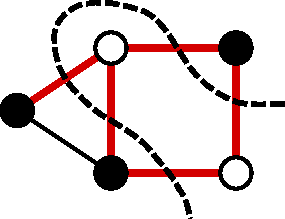
\includegraphics[width=.47\textwidth]{Max-cut.pdf}}
        \end{center}
    \end{figure}
\end{minipage}



\begin{minipage}{.55\linewidth}
    \theo{https://en.wikipedia.org/wiki/Prufer_sequence}
    {Prufer sequence}{
        Consider a labeled tree $ T $ with vertices's $ \{1, 2, ..., n\} $. At
        step $ i $, remove the leaf with the smallest label and set the $ i $th
        element of the \textit{Prüfer sequence} to be the label of this leaf's
        neighbour. Prove that a Prüfer sequence of length $ n-2 $ defines a Tree
        with length $ n $.

    }
\end{minipage}\hfill%
\begin{minipage}{.45\linewidth}
    \figdf{.4}{prufer_code_example}{${4,4,4,5}$}
\end{minipage}




\prob{https://artofproblemsolving.com/community/c6h5976p20088}
{German TST 2004 E7P3}{M}{
    We consider graphs with vertices colored black or white. ``Switching" a
    vertex means: coloring it black if it was formerly white, and coloring it
    white if it was formerly black.\\

    Consider a finite graph with all vertices colored white. Now, we can do the
    following operation: Switch a vertex and simultaneously switch all of its
    neighbours (i. e. all vertices connected to this vertex by an edge). Can we,
    just by performing this operation several times, obtain a graph with all
    vertices colored black?
}\label{problem:induction_type1_30}


\solu{A classical example of creating complex moves from counter cases.}


\prob{https://artofproblemsolving.com/community/c6h589936p3493453}
{ARO 2014 P9.8}{H}{
    In a country of $ n $ cities, an express train runs both ways between any
    two cities. For any train, ticket prices either direction are equal, but
    for any different routes these prices are different. Prove that the
    traveler can select the starting city, leave it and go on, successively, $
    n-1 $ trains, such that each fare is smaller than that of the previous
    fare. (A traveler can enter the same city several times.)
}\label{tickets}


\prob{https://artofproblemsolving.com/community/c6h364267}
{Generalization}{H}{
    Let $ A $ be a set of $ n $ points in the space. From the family of all
    segments with endpoints in $ A $ , $ q $ segments have been selected and
    colored yellow. Suppose that all yellow segments are of different length.
    Prove that there exists a polygonal line composed of $ m $ yellow
    segments, where $ m\geq\frac{2q}{n} $ , arranged in order of increasing
    length.
}\label{problem:constructive_algo_9}\label{problem:swapping_4}

\solu{
    Make one person go to every node. Then let the two people on the two sides
    of the most expensive edge swap their position. This ensures that every
    edge was used exactly 2 times. Using PHP, we have the desired result.
    Another solution is by 
    \autoref{theorem:mirsky_theorem}.
}



\prob{}
{}{E}{
    Given a bipartite graph, prove that the minimum number of colors required
    to color the edges of the graph such that no node is adjacent to $ 2 $
    edges of same color is the maximum degree of the graph.
}\label{problem:bipartite_graph_3}


\prob{}
{}{E}{
    For every bipartite graph prove that it's edges can be bicolored so that each
    node is adjacent to atmost $ \ceil{\dfrac{deg}{2}} $ edges of  any color.
}\label{problem:bipartite_graph_4}


\solu{Using the main property of a bipartite graph.}


\solu{After finding the cycle solution, to optimize it, we recall that we can find a Eulerian Path (if it exists) in $ O(V+E) $. Now we want to make the graph have a Eulerian path, so we add a vertice to both sides of the graph, and join them with odd vertices from the other side.}



\prob{https://artofproblemsolving.com/community/c6h446932}
{Turkey National MO 2002 P3}{HM}{
    Graph Airlines $(GA)$ operates flights between some of the cities
    of the Republic of Graphia. There are at least three $GA$ flights from each
    city, and it is possible to travel from any city in Graphia to any city in
    Graphia using $GA$ flights. $GA$ decides to discontinue some of its flights.
    Show that this can be done in such a way that it is still possible to travel
    between any two cities using $GA$ flights, yet at least $2/9$ of the cities
    have only one flight.

    \textbf{\Share\color{probC}Simplified:} In a connected graph, every
    vertex has degree at least $3$. Prove that some edges can be deleted to
    turn that graph into a tree with at least $\frac{2}{9}$ leaves. 

    \textbf{\Share\color{probC}Better Approximation:} We can actually achieve
    $\frac{1}{4}$ with careful construction.

    \index[strat]{Construction!Turkey NMO 2002 P3}
    \index[strat]{Bounding!Cost function!Turkey NMO 2002 P3}
}

\begin{solution}[dgrozev]
    First we construct a spanning tree $T$ that maximizes the number of leaves,
    then we bound the number. We define $G(V, E), n = \left|V\right| $ with
    the usual notations.\\

    Let $f: V \to V$. We initialize the tree by selecting a vertex $v$ by
    random, and adding it to $T$. We inductively add the vertices according to
    the following priority checks:

    \begin{enumerate}[label=\textbf{\boxed{\arabic*.}}, itemsep=5pt]
        \item If there is a vertex $v\not \in T$ that is connected to $u\in T$
            such that $u$ is not a leaf, then add $v, uv$ to $T$.
        \item If $u\in T$ is a leaf and there are two $v_1, v_2$ not in $T$
            that are connected to $u$, add $v_1, v_2$ and $uv_1, uv_2$ to $T$.
        \item If $u\in T$ is a leaf, and there is a $v$ which has two
            neighbors outside of $T$, then add $v, uv$ to $T$, and let $f(u)=v$.
        \item If $u\in T$ is a leaf, there is a $v \not \in T$ which is
            connected to at most one vertex outside $T$, and connected to
            $u'\in T$, then add $v, uv$ to $T$ and let $f(u) = u'$.
    \end{enumerate}
    This algorithm will add all the vertices to the tree. We now need to bound
    the number of leaves.\\

    Let $n_1, n_2, n_3$ be the set of vertices that have $1, 2$ and more than
    $3$ neighbors respectively. Since $f$ is a injection from the set $n_2$ to
    either $n_1$ or $n_3$, we have since $n = n_1+n_2+n_3$,
    \[n_2 \le n_1 + n_3,\quad n_2 \le \frac{n}{2}\]
    Bounding the number of edges gives us:
    \[\begin{aligned}
        2n-2 &\ge n_1 + 2n_2 + 3n_3\\
             &= n_1 + 3(n-n_1) - n_2\\
             &\ge 3n - 2n_1 - \frac{n}{2}\\
        \implies n_1 &\ge \frac{n}{4}+1
    \end{aligned}\]
\end{solution}

\begin{solution}[\href{http://wwwmayr.in.tum.de/konferenzen/Jass08/courses/1/gravin/Gravin_Slides.pdf}{Paper}]
    The construction is the same as before. But we define a different cost
    fuction $f$ to bound our leaves count. Let $D(T)$ be the number of leaves in
    $T$ which doesn't have a neighbor outside of $T$. Let $L(T)$ be the number of
    all leaves, and $V(T)$ is the number of vertices of $T$. Then consider 
    \[\boxed{f(T) = 3L(T) + D(T) - V(T)}\] 
    We show that $f(T)$ is non decreasing in our construction. If it is, we
    will get by setting $f(T_0)$ for a one vertex and its neighbor tree $T_0$, 
    \[f(T) \ge f(T_0) \ge 3\times 3 +0 -4 = 5 \] 
    And since $D(T') = L(T')$ for a spanning tree $T'$, \[L(T') \ge \frac{N+5}{4}\] 
    We now check that for all of your steps in construction, $f(T)$ is non
    decreasing.
\end{solution}



\prob{https://artofproblemsolving.com/community/c6h100733p568964}{ISL 2005 C1}{E}{A house has an even number of lamps distributed among its rooms in such a way that there are at least three lamps in every room. Each lamp shares a switch with exactly one other lamp, not necessarily from the same room. Each change in the switch shared by two lamps changes their states simultaneously. Prove that for every initial state of the lamps there exists a sequence of changes in some of the switches at the end of which each room contains lamps which are on as well as lamps which are off.}\label{problem:divide_and_conquer_4}\label{problem:induction_type1_10}



\prob{https://artofproblemsolving.com/community/c6h597130p3543398}{ISL 2013 C3}{M}{A crazy physicist discovered a new kind of particle which he called an $ i $ -mon, after some of them mysteriously appeared in his lab. Some pairs of $ i $ -mons in the lab can be entangled, and each $ i $ -mon can participate in many entanglement relations. The physicist has found a way to perform the following two kinds of operations with these particles, one operation at a time.

    \begin{enumerate}

        \item If some $ i $ -mon is entangled with an odd number of other $ i $ -mons in the lab, then the physicist can destroy it.

        \item At any moment, he may double the whole family of $ i $ -mons in the lab by creating a copy $ I' $ of each $ i $ -mon $ I $. During this procedure, the two copies $ I' $ and $ J' $ become entangled if and only if the original $ i $ -mons $ I $ and $ J $ are entangled, and each copy $ I' $ becomes entangled with its original $ i $ -mon $ I $ ; no other entanglements occur or disappear at this moment.

    \end{enumerate}

    Prove that the physicist may apply a sequence of much operations resulting in a family of $ i $ -mons, no two of which are entangled.
}\label{problem:induction_type1_9}


\solu{As there are an integer number of $ i $ -mons, it is quite natural to use induction. We try to find an algorithm to reduce the number of particles.

Another way to do this is to consider the chromatic number of the graph. If we can show that this number reduces after some move, then we are done by induction.}



\prob{https://artofproblemsolving.com/community/c6h104152p586762}{ISL 2005 C2}{E}{A forest consists of rooted (i. e. oriented) trees. Each vertex of the forest is either a leaf or has two successors. A vertex $ v $ is called an extended successor of a vertex $ u $ if there is a chain of vertices's $ u_{0}=u , u_{1}, u_{2} \dots u_{t-1} , u_{t}=v $ with $ t>0 $ such that the vertex $ u_{i+1} $ is a successor of the vertex $ u_{i} $ for every integer $ i $ with $ 0\leq i\leq t-1 $.\\

    Let $ k $ be a nonnegative integer. A vertex is called dynastic if it has two successors and each of these successors has at least $ k $ extended successors.\\

Prove that if the forest has $ n $ vertices, then there are at most $ \frac{n}{k+2} $ dynastic vertices.}\label{problem:induction_type1_8}

\solu{Trying to apply induction, we realize the bound is very loosy. That's why when we try to add in the inductive step, the value becomes larger than the bound. To stop that overflow, we tighten the bound.}

\solu{The second and dummy approach is to first doing some smaller cases, finding small infos, taking the root, seeing that the bound doesnt work, but it would work if one of the successors of the root would have exactly or less than $ 2k+3 $ successors. As we can't always guarantee that, we look for such a vertex with $ 2k+3 $ successors. We do some work with it and by induction its done.}



\prob{https://artofproblemsolving.com/community/c6h1441121p8200413}{All Russia 2017 9.1}{E}{In a country some cities are connected by oneway flights (There are no more then one flight between two cities). City $ A $ called "available" for city $ B $ , if there is flight from $ B $ to $ A $ , maybe with some transfers. It is known, that for every 2 cities $ P $ and $ Q $ exist city $ R $ , such that $ P $ and $ Q $ are available from $ R $. Prove, that exist city $ A $ , such that every city is available for $ A $.}\label{problem:induction_type1_17}



\prob{www.google.com}{Jacob Tsimerman Induction}{E}{There are $ 2010 $ ninjas in the village of Konoha (what? Ninjas are cool.) Certain ninjas are friends, but it is known that there do not exist $ 3 $ ninjas such that they are all pairwise friends. Find the maximum possible number of pairs of friends.(If ninja $ A $ is friends with ninja $ B $ , then ninja $ B $ is also friends with ninja $ A $.)}\label{problem:induction_type1_16}


\prob{https://artofproblemsolving.com/community/c6h420430p2374818}{USA TST 2011 D3P2}{M}{Let $n \geq 1$ be an integer, and let $S$ be a set of integer pairs $(a,b)$ with $1 \leq a < b \leq 2^n$. Assume $|S| > n \cdot 2^{n+1}$. Prove that there exists four integers $a < b < c < d$ such that $S$ contains all three pairs $(a,c)$, $(b,d)$ and $(a,d)$.}\label{problem:induction_type1_19}

\solu{Using Induction to the first and last half of the set $ S $ shows us the \hrf{finding_the_tough_nut}{hardest part} of the problem. Then ordering the left and right elements with some sort of hierarchy is all the work left to do.}




\prob{https://artofproblemsolving.com/community/c6h1480703p8639274}{ISL 2016 C6}{H}{There are $ n \geq 3 $ islands in a city. Initially, the ferry company offers some routes between some pairs of islands so that it is impossible to divide the islands into two groups such that no two islands in different groups are connected by a ferry route.\\

    After each year, the ferry company will close a ferry route between some two islands $ X $ and $ Y $. At the same time, in order to maintain its service, the company will open new routes according to the following rule: for any island which is connected to a ferry route to exactly one of $ X $ and $ Y $, a new route between this island and the other of $ X $ and $ Y $ is added.\\

Suppose at any moment, if we partition all islands into two nonempty groups in any way, then it is known that the ferry company will close a certain route connecting two islands from the two groups after some years. Prove that after some years there will be an island which is connected to all other islands by ferry routes.}\label{problem:induction_type1_11}

\solu{It is only natural to use induction on this kinda problems. After some trying, we see that if we remove $ 1 $ node, We get to nowhere, but if we remove $ 2 $ nodes, we get something interesting. So now focus on those two nodes and the rest of the nodes separately. Its not hard from there.}

\solu{As it seems, the separation of the graph was the main observation. We can call this trick \hl{Bringing Order in the Chaos}.}



\prob{https://artofproblemsolving.com/community/c6h535003p3067563}{ARO 2013 P9.5}{M (8/10)}{$ 2n $ real numbers with a positive sum are aligned in a circle. For each of the numbers, we can see there are two sets of $ n $ numbers such that this number is on the end. Prove that at least one of the numbers has a positive sum for both of these two sets.}\label{problem:graph_representation_4}\label{problem:minus_constant_2}

\solu{Since there is nothing specfic about the sum, we may safely assume that it is $ 0 $, because (1) probably it works, and (2) it makes things more convenient. How we do that? we decrease every number by the average.\\

    Now, Consider every block of $ n $ consecutive blockes of numbers. When are two blocks connected? When they share the same end. What if we consider them as vertices, and this ``connectivity'' as edges? We see that cycles pop out.\\

And we make use of the fact that our sum is $ 0 $. So signs are sure to bet flipped at the opposite side, and there are odd and even -ness in cycles that we can use.}




\prob{https://artofproblemsolving.com/community/c6h420424p2374799}{USA TST 2011 P2}{HM (9/10)}{In the nation of Onewaynia, certain pairs of cities are connected by roads. Every road connects exactly two cities (roads are allowed to cross each other, e.g., via bridges). Some roads have a traffic capacity of 1 unit and other roads have a traffic capacity of $ 2 $ units. However, on every road, traffic is only allowed to travel in one direction. It is known that for every city, the sum of the capacities of the roads connected to it is always odd. The transportation minister needs to assign a direction to every road. Prove that he can do it in such a way that for every city, the difference between the sum of the capacities of roads entering the city and the sum of the capacities of roads leaving the city is always exactly one.}\label{problem:divide_and_conquer_1}\label{problem:induction_type2_3}

\solu{As there are two types of subgraph, $ 1 $ -type and $ 2 $ -type. By some work-arounds, we see that we have to work distinctly in both types of graphs. Firstly, if we work in type- $ 1 $ , we see after making a path from node $ x, y $ , the degrees of $ x, y $ will be $ \{1, -1\} $ and the degrees of other nodes on the path will be the same. After that, we make every nodes have degree either $ \{1, -1\} $. So after this operation we remove the $ 1 $ -edges. Now, when dealing with the type- $ 2 $ sub-graph. Start over from zero, we see that when making a path between nodes $ x, y $ the degree of those two changes parity, and other nodes on the path stays the same. So select two odd nodes.... }

\solu{Dealing with two different kind of edges simultaneously is messy, so we work with graph $ 1 $ and graph $ 2 $ differently. Now on both graphs, we can remove cycles. And in graph $ 2 $ , we see that we can remove any big paths if there is a edge $ 1 $ joining the two endpoints. Since if the new graph works then the previous graph works too. [Several cases to show here] And if there is no edge joining the two endpoints, replace the path by joining the two endpoints by a edge $ 2 $.\\

Now there are only edge $ 1 $ s, and lone edge $ 2 $ s. Now dividing the graph $ 1 $ into paths of edge $ 1 $ , and dealing with several small cases, we are done.}



\prob{https://artofproblemsolving.com/community/c6h276187p1494557}{Iran TST 2009 P6}{E-M (9/10)}{We have a closed path that goes from one vertex to another neighboring vertex, on the vertices of a $ n\times n$ square which pass throgugh each vertex exactly once. Prove that we have two adjacent vertices such that if we cut the path at these two points then the length of each open paths is at least $ n^2/4 $.}

\solu{Draw a path, doesn't it look like a snake? Now can we relate the area of the tiled path with its perimeter? If we could do that, we would be able to replace two neighboring vertices by an edge inside the path, which seems to make the problem simpler.}



\prob{https://math.stackexchange.com/questions/1439430/algorithm-to-uniquely-determine-a-number-using-two-adjacent-digits}{OC Chap2 P2}{M (6/10)}{Arutyun and Amayak perform a magic trick as follows. A spectator writes down on a board a sequence of $ N $ (decimal) digits. Amayak covers two adjacent digits by a black disc. Then Arutyun comes and says both closed digits (and their order). For which minimal $ N $ can this trick always work? NOTE: Arutyun and Amayak have a strategy determined beforehand.}\label{problem:bijection_2}\label{problem:hall_marriage_1}

\solu{We have to actually find a bijection between all of the combinations the spectator can create, and all of the combinations that Arutyun might see when he comes back. Which tells us to use ``Perfect Matching" tricks.}

\solu{Existential proof: for this trick to always work, they have to make a bijection from a set of $ N $ digits with two covered, to an unique set of $ N $ digits. Consider a bijection from the set of $ 0-9 $ strings with length $ N $ to the set of $ 0-9 $ strings with length $ N $ with $ 2 $ adjacent digits unknown. There exist a bijection iff the two sets satisfy Hall's Marriage Theorem. By double counting we get the value of $ N $ from here.}



\prob{}{Simurgh 2019 P3}{E}{Call a graph \textit{symmetric}, if one can put its vertices on the plane such that it becomes symmetric wrt a line (which doesn't pass through any vertex). Find the minimum value of $ k $ such that (the edges of) every graph on $ 100 $ vertices, can be decomposed into $ k $ symmetric subgraph.}



\prob{https://artofproblemsolving.com/community/c6h2019175p14186360}
{RMM 2020 P3}{MH}{
    Let $n\ge 3$ be an integer. In a country there are $n$ airports and $n$
    airlines operating two-way flights. For each airline, there is an odd
    integer $m\ge 3$, and $m$ distinct airports $c_1, \dots, c_m$, where the
    flights offered by the airline are exactly those between the following
    pairs of airports: $c_1$ and $c_2$; $c_2$ and $c_3$; $\dots$ ; $c_{m-1}$
    and $c_m$; $c_m$ and $c_1$.

    Prove that there is a closed route consisting of an odd number of flights
    where no two flights are operated by the same airline.

    \index[strat]{Induction!Special!RMM 2020 P3}
    \index[strat]{Local!Add One by One!RMM 2020 P3}
    \index[strat]{Graph!Hall Marriage!RMM 2020 P3}
    \index[strat]{Graph!Bipartite!RMM 2020 P3}
}

\solu{[Weird Induction]
    Fix one vertice, merge all neighbors with it that has a unique airline between them.
}

\solu{[Element of Time]
    Add one edge from each cycle one at a time, without creating a cycle. Our objective is to show that when we reach the maximum stage where one edge creates a cycle, that cycle is of odd length.
}
